\clearpage
\section{Discussion}
\label{sec:discussion}

\subsection{Interpretation of Results}
\subsubsection{Substitutional Effects and Expanding of Bicycle Fleet to Less Accessible Areas}

% both bicycles and pt improve
Analyzing the mean and quantiles of the optimal X-minute city in Table \ref{tab:optimal_x_minute_city_metric} for each hexagon and scenario, revealed that both bicycle sharing and public transport, when added to another scenario, can decrease the time it takes to reach all necessities.
The average improvement that comes from adding bicycle to the mix varies between 1:16 minute and 1:36 and the average improvement that comes from adding public transport to the mix varies between 0:56 and 1:18.
Therefore, we can say that both methods are effective in improving accessibility over walking.


\paragraph{Public Transport Effectiveness}
% pt for remote areas of low accessiblity 
Various findings lead us to the conclusion that while public transport effective in improving accessibility, the most benefit is generated in remote suburban areas, that have a low density of POIs and that are located near to stops connected to high frequency public transport lines.
In addition, we find that public transport, compared to bicycle sharing is more costly.


In Figure \ref{fig:mean_time_per_cost} we can clearly see that when users are able to afford a short public transport trip (cost of 2.20), their accessibility to POIs increases.


% pt for areas of low accessiblity 
Firstly, the improvement seen by adding public transport mainly comes from areas with low accessibility as seen in Table \ref{tab:optimal_x_minute_city_metric} and Figure \ref{fig:optimal_x_minute_city_metric}.
These areas, or hexagons, are likely far from POIs, and we suspect that  public transport helps by covering these longer distances. 
However, in areas where it's already easy to get to these places, adding public transport might not make a big difference. 
This is because using public transport often involves extra steps: walking to the bus or train stop and waiting for it to arrive. 
How much this extra time matters depends on how long the whole trip is.
For short trips, the time spent getting to and waiting for public transport could be a large part of the travel time, making it less useful. 
But for longer trips, especially in the areas that were hard to reach before, this extra time is a smaller part of the journey. 
This makes public transport more beneficial for these longer trips. 

% pt actually better than bicycle for 20% worst
Secondly, in Figure \ref{fig:optimal_x_minute_city_metric} we see the full distribution of the optimal X-minute city metric for each scenario.
Notably, while public transport is worse than bicycle for the 80\% most accessible hexagons it shows a distinct advantage over bicycle sharing beyond the 80\% quantile, facilitating faster access in less accessible areas. 
The reason for this change in effectiveness between public transport and bicycle sharing is linked to how bicycle sharing is set up in Cologne. 
With the majority of bicycles available in the city center's "Flex-Zone", suburban areas have fewer bicycles as they can only be found at stations.
Consequently, the least accessible hexagons, typically situated in suburban regions, experience low to no availability of bicycles, which explains the superiority of public transport in these areas. 

% rath/neumar is reachable better by pt
This hypothesis is further supported when comparing the optimal X-minute city metric spatially between public transport and bicycle sharing, as seen in Figure \ref{fig:bicycle_optimal_map} and \ref{fig:public_transport_optimal_map}.
We see the district of Rath/Neumar in the east, which shows low accessibility in general.
However, we can clearly see that public transport has an advantage over bicycle sharing in this remote area.

% pt only better at 90% pareto front
In addition, when investigating the cost and X-minute city metric Pareto fronts in Figure \ref{fig:quantile_time_per_cost}, we see that public transport is only able to yield larger improvements than bicycle sharing when considering only the 10\% worst accessible hexagons.

% cost stuff
Table \ref{tab:required_cost} and Figure \ref{fig:maximum_required_cost_for_x_minute_city} show that public transport's advantage at the least accessible hexagons comes at a cost.
As soon, as the benefits of public transport manifest, the cost also increases to 2.20€, which is obvious as public transport rides are always charged.
We can see, however, that is really rarely necessary to travel more than four stops, as the cost for that (3.20€) is only reached at the very end. 
The three- or four-step increases to the cost of 2.20€ and 3.20€ can be explained by the different sub-scenarios.
In some scenarios it might be only beneficial to use public transport later.

Looking at Figure \ref{fig:maximum_required_cost_for_x_minute_city} also clearly reveals the spatial usage pattern of public transport.
As already conjectured previously, we see that mostly public transport is used in remote locations outside the city, that we know have lower accessibility in general.

The single hexagons inside the cities seen in Figure \ref{fig:maximum_required_cost_for_x_minute_city} are most likely located very close to a public transport stop, enabling to use the public transport system without any loss of time.
Inside the city it seems to only be beneficial to use the public transport system to reach necessities when living near a stop.
However, outside the city the larger groups of hexagons indicate that using the public transport system is often faster than walking to the necessities, eventhough walking to the next stop requires some time.
This may be, because the density of the POIs is lower outside the city.

% comparison of usefulness of short and long trips
With the help of the cost and X-minute city metric Pareto fronts, we are able to evaluate the usefulness and cost-efficiency of short trips (those that travel no more than 4 stops) and long trips (those that travel more than 4 stops).
Figure \ref{fig:mean_time_per_cost} and Table \ref{tab:differences_in_mean_pareto_front} show that the improvement caused by the short trip tickets is on average 1.28 minutes, compared to the 0.074 minutes of long trip tickets, and therefore almost 20 times larger.
Different from what we previously assumed, long distance trips actually don't bring a lot of benefit.
However, we should note that just because it is not beneficial to travel more than four stops, this does not mean that trips associated with four stops or fewer don't travel long distances.
Especially in suburban areas, where public transport stops are more sparse than in the city center, it might very well be that trips with four stops or fewer still travel multiple kilometers.
When investigating the 25\% quantile and 75\% quantile Pareto fronts in Figure \ref{fig:quantile_time_per_cost}, there is no benefit of long distance tickets displayed.
Only when investigating the 90\% quantile Pareto front, the benefit is visible.
This indicates that long distance trips are only used for the absolute worst accessible hexagons.
% END 

\paragraph{Bicycle Sharing Effectiveness}
% intro
The implementation of bicycle sharing has shown to enhance accessibility in a broad spectrum of urban areas. 
This improvement is not limited to less connected zones but is also evident in areas already well-served by existing transport networks.
Additionally, bicycle sharing has shown to be more cost-efficient than public transport.


% bicycles improve in general
In Figure \ref{fig:mean_time_per_cost} we can clearly see that when users are able to afford a bicycle for 15 minutes (cost of 1€), their accessibility to POIs increases drastically.


As detailed in Table \ref{tab:optimal_x_minute_city_metric} and Figure \ref{fig:optimal_x_minute_city_metric}, the introduction of bicycle sharing yields benefits across almost all hexagons, offering a more uniform impact compared to public transport. 
It is particularly notable that bicycle sharing also yields improvements in already well-accessible areas. 
We think that this is due to the fact that bicycles have a lower overhead which in turn contributes significantly to their practicality in urban settings.
Firstly, the higher density of bicycle access points compared to public transport stops inherently reduces the initial distance required to access a mode of transport, which  facilitates quicker access to the transport system. 
Secondly, bicycles eliminate the waiting period often associated with public transport schedules, which means that once a user reaches a bicycle, they can immediately start their journey. 
This immediacy and ease of access render bicycles an effective solution for a more general scope than public transport.

Further, the data in Figure \ref{fig:optimal_x_minute_city_metric} reveals that in more accessible hexagons, combining bicycles with public transport offers greater advantages over using public transport alone. 
Interestingly, looking at least accessible hexagons, the disparity between these two scenarios narrows. 
This observation implies that in areas with very low accessibility, which are most likely remote areas, the addition of bicycles does not significantly enhance accessibility.
This trend is likely due to the limited availability of bicycles in these less accessible areas, underscoring the importance of equitable distribution in bicycle sharing systems.

We already hypothesized that the low utility for bicycle sharing in areas with low accessibility is linked to the low availability of bicycles in suburban areas, as the majority of bicycles is located in the "Flex-Zone".
This hypothesis gains further support when contrasting Figures \ref{fig:bicycle_optimal_map} and \ref{fig:walking_optimal_map}. 
Here, an improvement is observed in the bicycle scenario compared to walking, particularly within the "Flex-Zone" as shown in Figure \ref{fig:flex_zones}, which underscores the impact of the zone on accessibility patterns.

\begin{figure}
  \begin{center}
    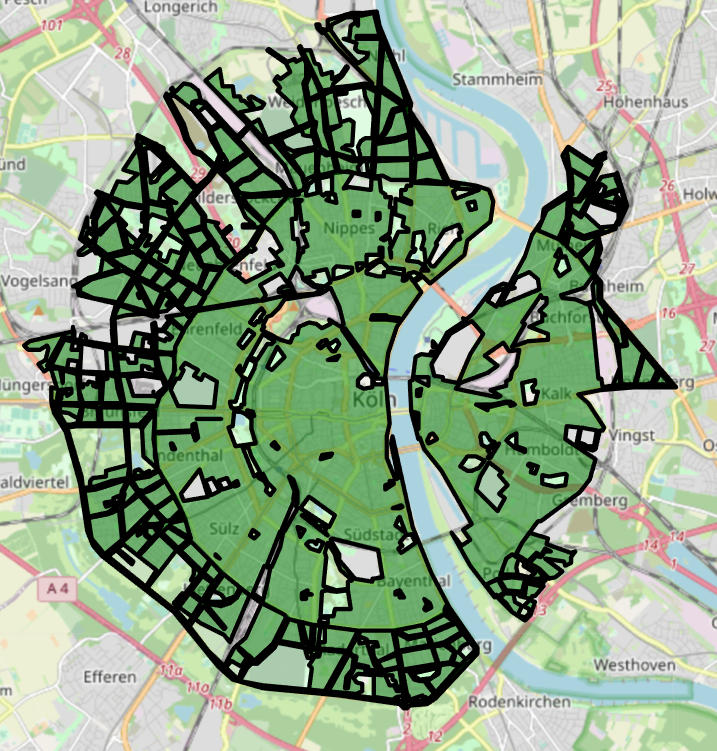
\includegraphics[width=0.50\textwidth]{Figures/discussion/flex_zones.png}
  \end{center}
  \caption{Next Bike's Flex Zones}
  \label{fig:flex_zones}
\end{figure}

% pt only better at 90% pareto front
Investigating the cost and X-minute city metric Pareto fronts in Figures \ref{fig:mean_time_per_cost} and \ref{fig:quantile_time_per_cost}, as well as, the corresponding values of improvement in Tables \ref{tab:differences_in_mean_pareto_front}, \ref{tab:differences_in_75_quantile_pareto_front} and \ref{tab:differences_in_90_quantile_pareto_front} shows that using a bicycle for 15 minutes always yields larger time gains than public transport except for the 10\% worst accessible hexagons.
This is a clear indicator for the superiority of bicycle sharing over public transport in terms of accessibility improvements, especially, when considering that the bicycle sharing infrastructure does not cover all of the considered area.


% cost stuff
Table \ref{tab:required_cost} and Figure \ref{fig:maximum_required_cost_for_x_minute_city} clearly indicate that bicycle sharing never costs more than public transport, if both are used.
We can also deduct this from the price of both and the fact that bicycles are never used more than 15 minutes.
We now that bicycles are never used for more than 15 minutes as the maximum cost, as seen in Table \ref{tab:required_cost} is 1.00€, which is the price for a 15-minute ride.
Meanwhile, the shortest possible public transport trip costs 2.20€, therefore as soon as public transport is used it always costs more than bicycles.
Nevertheless, this already shows that bicycle sharing is cheaper than public transport. 

In addition, knowing that bicycles never are used for more than 15-minute tells us that at any location where bicycles are available, Cologne is a 15-minute city.
This is a strong indicator that bicycle sharing is able to make regions 15-minute city regions.

Table \ref{tab:differences_in_mean_pareto_front} shows the average improvements of the X-minute city metric, at the cost points where public transport and bicycle sharing are used.
We see that bicycle sharing is on average more than 3 times more cost-efficient than public transport.
Further, investigating the differences at the 75\% and 90\% quantile Pareto fronts in Table \ref{tab:differences_in_75_quantile_pareto_front} and \ref{tab:differences_in_90_quantile_pareto_front}, shows that bicycle sharing always is more cost-efficient than public transport.
This again proves that expanding bicycle sharing zones to suburban areas might be more beneficial to residents, than improving public transport.

%END

% not sure where to put this
Another difference between bicycles and public transport is that they differ notably in their speed and route flexibility. 
Public transport typically travels faster than bicycles, which offers a clear advantage for covering long distances. 
This speed is particularly beneficial when some POIs are far away, as public transport can effectively bridge these larger gaps. 
However, the fixed routes of public transport mean that users may not always disembark close to their desired POI. 
In contrast, bicycles offer the flexibility of route choice, allowing users to tailor their journey to arrive nearer to the POI. 
This also aligns with the finding that public transport tends to be most effective for the least accessible hexagons, where distance to POIs is a significant factor.

% not sure where to put this
In general, bicycle sharing brings larger improvements than public transport, while remaining more cost-effective.
The improvements of bicycle sharing are effective for the most accessible regions, while the improvements of public transport are not.
This shows that extending the bicycle sharing system might be a good way to improve the accessibility in Cologne.

However, for the least accessible regions, public transport is more effective than bicycle sharing.
This most likely means that there are regions in the region of Cologne, where some categories of POIs are not present.
We suspect that those regions are characterized by low accessibility and low or no availability of bicycles.
In those regions public transport becomes more effective than bicycles, as it essentially allows to relocate to better areas.
In the spirit of the 15-minute city, it might be more desirable to fix the sparsity of POIs than to substitute public transport.
% end


\paragraph{Bicycle Sharing and Public Transport - Substitutes or Complements?}
% introduction of substitutional effects and complement I & II
As already mentioned we found clear evidence that bicycle sharing and public transport have a positive effect on accessibility according to the X-minute city metric.
It is, however, not clear whether these modes are substitutional to each other, meaning that one mode is able to compensate the other, or whether they are complements.
We potentially could observe two sorts of complementary effects.
The first (complement I) would be that bicycle sharing and public transport each are effective under different circumstances and in different areas.
If that's the case, one cannot replace the other, and each is necessary under specific circumstances.
The second effect (complement II) would be that sometimes bicycles sharing and public transport used together is necessary to improve vehicle sharing.
If that's the case, there both would be necessary to be employed together in order to achieve the highest accessibility.
Both effects can be described as complementary effects, and they are not mutually exclusive, which means that we can potentially observe both.


Table \ref{tab:optimal_x_minute_city_metric} shows that the combined scenario on average yields better accessibility than bicycle sharing and public transport alone.
This suggests that either complement I or complement II must be present.

% TODO: complement I
We see evidence for complement I in the observation that bicycle sharing is most effective for the 80\% more accessible hexagons, while public transport is mostly only effective for the 20\% least accessible hexagons.


% TODO: complement II

% TODO: implications of complement I & II
% implications
The presence of complement I should make us aware that the effectiveness of either mode is highly dependent on the spatial circumstances of the region.
Some regions might benefit more from bicycle sharing, while others benefit more from public transport.
It is therefore, necessary to analyze each region separately, to maximize the positive effect of sustainable modes of travel.
% implications END
%END



% not sure where to put this "conclusion"
Our findings lead to the conclusion that enhancing bicycle availability in areas with low accessibility could yield significant benefits.
Additionally, the observed dynamics suggest that bicycles are more advantageous in areas with low to medium accessibility, while public transport predominantly benefits the least accessible areas.
This again indicates that bicycles and public transport serve complementary, rather than substitutable, roles in urban mobility networks.
Therefore, removing one mode of transportation cannot be effectively compensated for by simply increasing the other, as each serves distinct and crucial functions in addressing different aspects of urban accessibility.


\subsubsection{Specific Recommendations for Cologne}

% Merkenich & rhine bridge
In Figure \ref{fig:optimal_map} we observed that Merkenich, which is located at the other side of the Rhine next to Leverkusen, is one of the least accessible regions in Cologne.
From Figure ???, we now that there are plenty of POIs for all categories in Leverkusen, which are very close to the problematic region.
This indicates a lack of mobility crossing the Rhine river.
As a bridge is already existing, we suggest providing a frequent public transport line to improve the accessibility in Merkenich.

% Rath/Neumar
In Figure \ref{fig:public_transport_optimal_map} we see that while the district of Rath/Neumar shows bad accessibility for all three scenarios, the accessibility in the public transport is better than that of walking and bicycle sharing.
This is not surprising, as this region is quite far away from POIs, which makes walking very slow.
Also, the region is not in NextBike's flex zone, which leads to a low availability of bicycles, explaining why the bicycle sharing scenario is as bad as walking here.
However, the city train line 9 runs through this region, which leads to a higher accessibility by public transport.

This fact shows us that, a high frequency public transport line from the city center to less accessible area can significantly improve accessibility.
It might be beneficial to create such lines to other less accessible regions in the north and south of Cologne's suburban areas.


\subsubsection{Cost per month}

A prevalent measure to incentivize the use of sustainable modes of transport are monthly tickets or subscriptions.
To measure whether the costs of these subscriptions are worth it, we will calculate the monthly cost incurred by the trips to all necessities.
To do so, we first collected how often people visit each of the categories we defined earlier.
The monthly number of visits per category can be seen in Table \ref{tab:monthly_visits}.

\begin{table}
  \caption{Number of monthly visits per category}
  \label{tab:monthly_visits}
  \begin{center}
    \begin{tabular}[c]{l|l}
      category & monthly visits \\
      \hline
      groceries & 12 \\
      education & 20 \\
      health & 0.42 \\
      banks & 9 \\
      parks & 2.4 \\
      sustenance & 6.12 \\
      shops & 4 \\
      \hline
    \end{tabular}
  \end{center}
\end{table}

The derivation of these numbers can be found in Appendix \ref{app:monthly_visits_per_category}


\subsubsection{Time Gains per Euro}

Table \ref{tab:differences_in_mean_pareto_front} shows how a minute of saved time costs for cycling and public transport, respectively.
The most cost-efficient variant, bicycle sharing, enables users to save 1.68 minutes per euro, which might not be worth it for most people.
The 1.68 minutes per euro spent, in other words means that to save a minute of time people have to spend around 62 cents.
Comparing this to the minimum wage in Germany of 12 euro per hour in 2022 \cite{federalstatisticalofficegermanyMinimumWages}, which is 20 cents per minute, shows that it takes around three minutes to make enough money to save one minute, which obviously is not worth it.
This means that currently on average the sustainable modes of travel are too expensive.

Even when looking at the least accessible regions (90\% quantile) separately in Figure \ref{fig:90_quantile_time_per_cost}, where we have the largest improvement possible, the most cost-efficient mode of transport, which is bicycle, only yields an improvement of two minutes per euro, which again does not result in a net positive for people who earn the minimum wage.

% TODO: more interpretation of Differences in  Pareto Front tables


\subsubsection{Uncertainty}

A deviation of one minute on average with a CV of $<10\%$ is acceptable.
It is interesting to note that bicycles suffer more from uncertainty than public transport. 
However, this might strongly depend on the choices of our sub-scenarios. 
For public transport we tried 08:00, 12:00 and 18:00.
We suspect that the variance for public transport would increase more drastically and eventually surpass the one of bicycle sharing if we choose more unusual times like midnight.
We should also note that the comparison of variances should be taken with caution as the method for selecting the sub-scenarios differ per scenario.
For bicycle sharing we employed a clustering method, while for public transport we made a qualitative choice. 

\subsubsection{Impact Of Sustainable Modes On 15-Minute Metric}

First, we should note that a majority of the problematic areas cannot be fixed by any sustainable mode, which is bad.
Next we see that bicycles sharing, and public transport alone are roughly of equal importance and are also able to fix more hexagons separately than together, which means that these modes are not substitutes.
We also see that the combined mode has only very little impact.

We suspect that this yellow ring is in an area where there are fewer POIs, but still a high availability of bicycles, that can compensate this sparsity.

The observation that orange is closer to the city center than yellow seems plausible as public transport can travel larger distances in shorter time than bicycle sharing, but require a larger overhead as stops are distributed sparser than bicycles and require a larger overhead as users might have to wait.

The unfixable regions mostly don't have bicycles near them, but they often have public transport nearby.
This suggests that bicycles are more effective than public transport to help a region become sub 15-minute.
